% !TEX root = main.tex

\begin{quote}
    \em
    \vphantom{}\marginnote{%
        \textbf{หมายเหตุ}\; โจทย์บางข้อที่ปรากฏอาจมีลักษณะเป็นคำถามปรนัย (มีตัวเลือก)
        เนื่องจากเป็นข้อจำกัดของระบบในการแข่งขันระดับ Audition
    }%
    \llap{\adfdownleafleft\;}สำหรับโจทย์ประเภท Ponder
    ผู้เข้าแข่งขันจะมีเวลาวิเคราะห์โจทย์และค้นหาคำตอบภายในเวลา 5 นาที\;
    สามารถใช้คอมพิวเตอร์เพื่อช่วยหาคำตอบได้อย่างเต็มที่
\end{quote}

\question{}

ธนาคารกสิกรไทยสาขา {\techjam} ได้ก่อสร้างอาคารสูง 1000 ชั้นเสร็จหมาด ๆ\; 
เจ้าหน้าที่ต้องการติดป้ายบอกชั้นตั้งแต่ชั้นที่ 1 ถึงชั้นที่ 1000 ชั้นละ 1 ชุด
โดยเลขแต่ละชุดเกิดจากการนำแผ่นกระดานที่มีเลขโดด 0 ถึง 9 
หลายแผ่นมาประกอบกันแล้วนำไปติดตามชั้นต่าง~ๆ\hrsp%
\sidenote{%
    \textbf{ตัวอย่าง} เช่นชั้นที่ 37 จะต้องใช้แผ่นกระดานเลขโดด 3 และ 7 อย่างละ 1 แผ่น
}

อยากทราบว่าเจ้าหน้าที่ต้องเตรียมแผ่นกระดานที่มีเลขโดด 9 ทั้งหมดกี่แผ่น
เพื่อนำมาติดป้ายให้ครบทุกชั้น?

\question{}

กำหนดให้มีต้นไม้ค้นหาแบบทวิภาค (Binary search tree) อยู่ต้นหนึ่ง 
ซึ่งประกอบไปด้วยจำนวนบางจำนวนที่อยู่ระหว่าง 1 กับ 100 ปรากฏอยู่

หากเราต้องการค้นหาข้อมูลซึ่งคือจำนวน 56 ภายในต้นไม้ข้างต้นนี้\;
ข้อใดต่อไปนี้เป็นลำดับการเกิด tree traversal ที่เริ่มต้นจากราก (root) เพื่อค้นห้าข้อมูลดังกล่าว
ที่ไม่สามารถเกิดขึ้นได้?

\begin{multicols}{2}
\begin{enumerate}[label={$\Circle$}]
\item 7, 82, 46, 66, 43, 58, 56
\item 92, 13, 66, 34, 61, 41, 56
\item 13, 77, 62, 41, 59, 57, 56
\item 77, 11, 72, 59, 13, 52, 56
\end{enumerate}
\end{multicols}

\question{}

ในบรรดาจำนวนเต็มตั้งแต่ 1 ถึง 1000 มีกี่จำนวนซึ่งมีผลรวมเลขโดดที่ไม่มีเลขโดด 1 
ปรากฏภายในผลรวมเลขโดดนั้นเลย?\hrsp%
\sidenote[][-\baselineskip]{%
    \textbf{ตัวอย่าง} เพื่อความชัดเจน
    \begin{itemize}
        \item เลข 123 มีผลรวมเลขโดดคือ $\mathrm{1+2+3=6}$ ซึ่ง\uline{ไม่มี}เลขโดด $\mathrm{1}$ อยู่ใน $\mathrm{6}$
        \item เลข 67 มีผลรวมเลขโดคือ $\mathrm{6+7=13}$ ซึ่ง\uline{มี}เลขโดด $\mathrm{1}$ อยู่ใน $\mathrm{13}$
    \end{itemize}    
}


\question{}

กำหนดให้มีจำนวน 6 จำนวน ได้แก่ 1, 2, 5, 6, 7, 9 
ให้นำจำนวนเหล่านี้มา ``บวก{\hrsp--\hrsp}ลบ{\hrsp--\hrsp}คูณ{\hrsp--\hrsp}หาร'' 
ให้ได้จำนวน 258 โดยที่มีเงื่อนไขดังนี้
\begin{itemize}
    \item จะใช้ $+, -, \times, \div$ อย่างไรก็ได้ และจะจัดกลุ่มหรือใส่วงเล็บอย่างไรก็ได้
    \item จะใช้ตัวเลขในลำดับใดก็ได้ แต่ต้องใช้ตัวเลขทุกตัว ตัวละหนึ่งครั้งพอดี
\end{itemize}

\noindent
จงหาวิธีการจัดนิพจน์ให้กับจำนวนทั้งหมดข้างต้น เพื่อให้ได้ผลลัพธ์ตามที่ต้องการ?


\newpage
\question{\label{q:ponder_northeast_audition_sqroot}}

จงพิจารณาโปรแกรมดังต่อไปนี้\,\sidenote[][6.15\baselineskip]{%
   \textbf{หมายเหตุ}\; \lstinline{floor} 
   คือฟังก์ชันที่ปัดเศษของจำนวนเต็มทิ้งให้กลายเป็นจำนวนเต็มที่มากที่สุดที่น้อยกว่าหรือเท่ากับจำนวนเดิม
}
\begin{lstlisting}
function mystery_<%\ref*{q:ponder_northeast_audition_sqroot}%>(n):
   # n <%\codecmt เป็นจำนวนเต็มที่ไม่ติดลบ%>
   lb := 0
   ub := n
   loop:
      attempt := floor((lb + ub) / 2)
      if n < attempt^2:
         ub := attempt - 1
      elseif n >= (attempt + 1)^2:
         lb := attempt + 1
      else: 
         break loop and return attempt
      end
   end
end
\end{lstlisting}
โปรแกรมข้างต้นทำหน้าที่ตามที่ระบุในข้อใดต่อไปนี้?

\begin{itemize}[label={$\Circle$}]
\item ฟังก์ชัน square root แต่ปัดเศษเป็นจำนวนเต็มที่ใกล้ที่สุดเสมอ\\ (round to nearest integer)
\item ฟังก์ชัน square root แต่ปัดเศษทิ้งเป็นจำนวนเต็มเสมอ (round down)
\item ฟังก์ชัน square root แต่ปัดเศษขึ้นเป็นจำนวนเต็มเสมอ (round up)
\item ฟังก์ชัน square root แต่เศษอาจถูกปัดขึ้นหรือลงอย่างไรก็ได้ ไม่สามารถคาดเดาได้
\item ฟังก์ชันติด infinite loop ไม่รู้จบ
\end{itemize}

\question{}

กำหนดให้ \lstinline{A} เป็น Array ของเลขจำนวนเต็มดังต่อไปนี้
\begin{center}
    \lstinline{A = [133, 60, 96, 130, 125, 65, 482, 88, 220, 165, 25, 45]}
\end{center}

จงเลือกจำนวน 3 จำนวนที่ไม่ซ้ำกันจาก \lstinline{A} แล้วหาผลคูณที่ลงท้ายด้วยเลขโดด 0 เยอะที่สุด
\uline{ผลคูณดังกล่าวมีค่าเท่าใด}?

\question{}

กำหนดให้ \lstinline{rand7()} เป็นฟังก์ชันที่สุ่มจำนวนเต็มในช่วงตั้งแต่ 1 ถึง 7 ด้วยความน่าจะเป็นเท่า ๆ กัน

ให้พิจารณานิพจน์ดังต่อไปนี้\hrsp%
\sidenote[][1.65\baselineskip]{%
    \textbf{หมายเหตุ}\; binary operator \lstinline{mod} 
    คือการหารที่เอาเฉพาะเศษเป็นผลลัพธ์ของนิพจน์นั้น เช่น \lstinline{13 mod 3 = 1}
}
ที่สุ่มจำนวนเต็ม 1 จำนวนในช่วงตั้งแต่ 1 ถึง 11
\begin{center}
    \lstinline{((rand7() + rand7()) mod 11) + 1}
\end{center}

อยากทราบว่า output ของนิพจน์ข้างต้นที่เป็นไปได้มากที่สุด มีค่าเท่าใด?


\newpage
\question{}

กำหนดให้มี input ทั้งสิ้น 1 จำนวน ได้แก่จำนวนจริง $x$

จาก input ข้างต้นนี้ เป้าหมายคือการคำนวณค่าของ $x^n$ โดยที่ $n$ เป็นจำนวนเต็มบวก  
โดยใช้ operation การคูณเป็น\uline{จำนวนครั้งน้อยที่สุด} ภายใต้เงื่อนไขดังต่อไปนี้
\begin{itemize}
\item อนุญาตให้ใช้เฉพาะ operation การคูณ
\item อนุญาตให้นำผลคูณที่เกิดขึ้นก่อนหน้านั้น\uline{ระหว่างการคำนวณ}
    มาใช้เป็นตัวตั้งหรือตัวคูณของการคูณครั้งถัดไปได้\hrsp%
    \sidenote[][-\baselineskip]{%
        \textbf{ยกตัวอย่าง}\; สมมติว่าเราต้องการคำนวณ $x^n$ ในกรณีที่ $n = \mathrm{6}$ 
        เราจะใช้การคูณ\uline{น้อยที่สุด}เพียง 3 ครั้งเท่านั้น เขียนเป็นขั้นตอนวิธีได้ดังนี้
        \begin{flushleft}
            \quad\lstinline{r_1 := x * x      # => x^2} \\
            \quad\lstinline{r_2 := r_1 * r_1  # => x^4} \\
            \quad\lstinline{r_3 := r_1 * r_2  # => x^6}
        \end{flushleft}

        สังเกตว่า จากข้อมูล $x$ ที่เราทราบ เราจะคำนวณหาค่าของ $x^\mathrm{2}$, $x^\mathrm{4}$ 
        และ $x^\mathrm{6}$ ตามลำดับ\;
        นอกเหนือจากวิธีนี้ ยังมีวิธีอื่นอีก เช่น การคำนวณหา $x^\mathrm{2}$, $x^\mathrm{3}$ 
        และ $x^\mathrm{6}$ ตามลำดับ
    }
    (หมายความว่า เรามีการ\uline{จดบันทึก}ผลการคูณที่เกิดขึ้นทั้งหมด 
    คล้ายกับ history tape ในเครื่องคิดเลขของนักบัญชี)
\end{itemize}

\noindent
\textbf{\uline{โจทย์}} การคำนวณหาค่าของ $x^n$ ในกรณีที่ $n=\mathrm{125}$ 
(นั่นคือให้คำนวณค่าของ $x^\mathrm{125}$) จะต้องใช้ operation การคูณเป็นจำนวน\uline{น้อยที่สุด}กี่ครั้ง? 
และการคูณในแต่ละขั้นนั้นจะคำนวณ $x^{???}$ อะไรบ้าง\uline{ตามลำดับ}?\; (ให้ตอบมา 1 วิธี)

\question{}

กำหนดให้มี input ทั้งสิ้น 3 จำนวน ได้แก่จำนวนจริง $x$, $y$ และ $z$

จาก input ข้างต้นนี้ เป้าหมายคือการคำนวณค่าของนิพจน์ $ax + by + cz$
โดยที่ $a$, $b$ และ $c$ เป็นค่าคงที่จำนวนเต็มที่ไม่ติดลบ 
โดยใช้ operation การบวกเป็น\uline{จำนวนครั้งน้อยที่สุด}\;
ภายใต้เงื่อนไขดังต่อไปนี้

\begin{itemize}
    \item อนุญาตให้ใช้เฉพาะ operation การบวก
    \item อนุญาตให้นำผลบวกที่เกิดขึ้นก่อนหน้านั้น\uline{ระหว่างการคำนวณ}
        มาใช้เป็นตัวตั้งหรือตัวบวกของการบวกครั้งถัดไปได้\hrsp%
        (หมายความว่า เรามีการ\uline{จดบันทึก}ผลการบวกที่เกิดขึ้นทั้งหมด 
        คล้ายกับ history tape ในเครื่องคิดเลขของนักบัญชี)
\end{itemize}

\noindent
\textbf{\uline{ตัวอย่าง}} สมมติว่าเราต้องการคำนวณ $x + \mathrm{2}y + \mathrm{3}z$ ในเคสทั่วไป
เราอาจคำนวณตามลำดับในสมการ $x + y + y + z + z + z$ ซึ่งใช้การบวกทั้งสิ้น 5 ครั้ง\; 
แต่เนื่องจากเงื่อนไขอนุญาตให้นำผลบวกก่อนหน้ามาใช้งานได้ เราสามารถใช้การบวกน้อยที่สุดเพียง 4 ครั้งเท่านั้น
ซึ่งเขียนเป็นขั้นตอนวิธีได้ดังนี้
\begin{lstlisting}
r_1 := y + z       # => y + z
r_2 := r_1 + r_1   # => 2y + 2z
r_3 := r_2 + z     # => 2y + 3z
r_4 := r_3 + x     # => x + 2y + 3z
\end{lstlisting}

\noindent
\textbf{\uline{โจทย์}} การคำนวณหาค่าของ $x + \mathrm{4}y + \mathrm{9}z$ จาก input $x$, $y$ และ $z$ 
จะต้องใช้ operation การบวกเป็นจำนวน\uline{น้อยที่สุด}กี่ครั้ง?

\question{}

สมมติว่าเรามีกองแท่งไม้ 5000 แท่ง แท่งไม้แต่ละแท่งมีความยาว 1, 2, 3, \ldots, 5000 หน่วยตามลำดับ\;
เราต้องการสร้างสามเหลี่ยมที่มี\uline{พื้นที่ภายในมากกว่าศูนย์}\hrsp%
\sidenote[][-\baselineskip]{%
    สามเหลี่ยมใด ๆ ที่มีพื้นที่มากกว่าศูนย์จะต้องมีผลรวมความยาวของด้าน 2 ด้านใด ๆ ยาวกว่าด้านที่สามเสมอ เช่น
    \begin{itemize}
        \item 3, 4, 5 ประกอบเป็นความยาวด้านของสามเหลี่ยม\uline{ได้}
        \item 1, 3, 5 ประกอบเป็นความยาวด้านของสามเหลี่ยม\uline{ไม่ได้} เพราะ $\mathrm{1 + 3 < 5}$
        \item 1, 2, 3 ประกอบเป็นความยาวด้านของสามเหลี่ยมได้ แต่จะมี\uline{พื้นที่เท่ากับ 0}
    \end{itemize}
}
โดยการหยิบแท่งไม้จากกองดังกล่าวมา 3 แท่งมาประกอบกัน

อยากทราบว่าเราจะมีวิธีเลือกหยิบแท่งไม้ 3 แท่งจากกองดังกล่าว
ประกอบให้กลายเป็นสามเหลี่ยมที่มีพื้นที่มากกว่าศูนย์ได้กี่วิธี?

\textbf{หมายเหตุ}\; ข้อนี้อาจต้องใช้ 64-bit integer


\newpage
\question{}

จงพิจารณาโปรแกรมดังต่อไปนี้
\begin{lstlisting}
function f(n):
    if n ≤ 1 then:
        return 1
    else:
        x = f(n/2)
        y = f(n/2)
        return g(n, x, y)
    end
end
\end{lstlisting}

หากกำหนดให้ time complexity ของฟังก์ชัน \lstinline{g(n, ·, ·)} คือ $O(\mathtt{n})$ 
แล้วจงคำนวณหา time complexity ของฟังก์ชัน \lstinline{f(n)}

\question{}

จงพิจารณาโปรแกรมดังต่อไปนี้
\begin{lstlisting}
function foo(A):
    n := A.length()
    bar(A, 0, n-1)
end

function bar(A, lo, hi):
    if hi - lo ≤ 31 then:
        return spin(A, lo, hi)
    end
    mid := select an integer strictly between <%\SuppressNumber%>
           lo and hi uniformly at random <%\ReactivateNumber%>
    return bar(A, lo, mid) + bar(A, mid, hi)
end

function spin(A, lo, hi):
    count := 0
    for i := lo to hi-1 do:
        for j := i + 1 to hi do:
            if A[i] > A[j] then count := count + 1
        end
    end
    return count
end
\end{lstlisting}

หากกำหนดให้ฟังก์ชัน \lstinline{foo(A)} ในโปรแกรมข้างต้นมี input argument 
คือ array \lstinline{A} ของจำนวนเต็มที่มีความยาว \lstinline{n} ตัวแล้ว
จงวิเคราะห์เพื่อคํานวณหา Worst-case time complexity และ Average-case time complexity 
ของฟังก์ชัน \lstinline{foo} ในรูปของ \lstinline{n}


\newpage
\question{}

นายกสิกรเขียนอักขระภาษาอังกฤษ 1 ตัว ลงบนแต่ละหน้าของเหรียญ 4 เหรียญ โดยไม่มีตัวอักขระตัวใดซ้ำกันเลย
จากนั้นเขาโยนเหรียญทั้ง 4 เหรียญลงบนโต๊ะอย่างสุ่ม แล้วนำอักขระบนเหรียญด้านที่หงายมาเรียงเป็นคำ
ทำอย่างนี้ทั้งหมด 3 ครั้ง สะกดได้คำว่า ``BOAT'', ``NODE'' และ ``RANT'' ตามลำดับ

อยากทราบว่า คำใด\uline{บ้าง}ต่อไปนี้ที่ไม่สามารถสะกดจากอักขระที่ปรากฏบนเหรียญได้?
\begin{multicols}{4}
\begin{itemize}[label={$\square$}]
\item BART
\item DONE
\item BORE
\item NEAR
\end{itemize}
\end{multicols}

\question{}

นายกสิกรเข้าร่วมในงานประมูลทะเบียนรถหมวด ``ฃฅ'' 
ซึ่งมีการเปิดประมูลเลขทะเบียนรถทุกหมายเลข ตั้งแต่ 1 จนถึง 9999

นายกสิกรเคยได้ยินจากหมอดูหลายท่านว่า หากต้องการให้ชีวิตมั่งคั่งร่ำรวย จะต้องมี ``ผลรวมเลขโดดสุดท้าย''\hrsp%
\sidenote{%
    ผลรวมเลขโดดสุดท้าย คือการหาผลรวมเลขโดดของจำนวนจำนวนหนึ่ง
    ซ้ำ ๆ กันไปเรื่อย ๆ จนกว่าจะเหลือเลขโดดเพียงตัวเดียว
}
เป็น 8 เช่น
\begin{itemize}[before*=\small]
    \item ป้ายทะเบียน 7595 \uline{เป็นป้ายทะเบียนมั่งคั่ง} \\
        เพราะ $\mathrm{7 + 5 + 9 + 5 = 26} \;\Longrightarrow\; \mathrm{2 + 6 = 8}$
    \item แต่ป้ายทะเบียน 7777 \uline{ไม่มั่งคั่ง} \\
        เพราะ $\mathrm{7 + 7 + 7 + 7 = 28} \;\Longrightarrow\; \mathrm{2 + 8 = 10} \;\Longrightarrow\; \mathrm{1 + 0 = 1 \neq 8}$
\end{itemize}

จงคำนวณว่า ในบรรดาป้ายทะเบียนในเปิดประมูลทั้งหมดในหมวด ``ฃฅ'' ในวันนี้ 
จะมีป้ายทะเบียนมั่งคั่งเป็นจำนวนกี่ป้าย?

\question{}

จงหาผลรวมของจำนวนทุกจำนวนที่ปรากฏในตารางดังต่อไปนี้
\[
    \footnotesize
    \begin{bmatrix}
        1 & 2 & 3 & \cdots & \cdots & 15000 \\
        2 & 3 & 4 & \cdots & \cdots & 15001 \\
        3 & 4 & 5 & \cdots & \cdots & 15002 \\
        \vdots & \vdots & \vdots & \ddots & & \vdots \\
        \vdots & \vdots & \vdots & & \ddots & \vdots \\
        15000 & 15001 & 15002 & \cdots & \cdots & 29999 \\
    \end{bmatrix}_{15000 \times 15000}
\]

\textbf{หมายเหตุ}\; ข้อนี้อาจต้องใช้ 64-bit integer
\question{}

กำหนดให้มีนาฬิกาดิจิทัลอยู่เรือนหนึ่ง มีลักษณะเป็น 24-hour clock
ที่แสดงผลในรูปแบบ \texttt{HH:MM:SS} ตั้งแต่เวลา \texttt{00:00:00} ไปจนถึง \texttt{23:59:59}

\medskip\noindent
\textbf{\uline{นิยาม}}\;
เวลา ณ วินาทีหนึ่ง ๆ จะเป็น ``เวลาเลขสวย'' ก็ต่อเมื่อการแสดงผลบนหน้าปัดนาฬิกา%
ประกอบไปด้วยเลขโดดที่แตกต่างกัน\uline{ไม่เกิน 2 ตัว}เท่านั้น ยกตัวอย่างเช่น
\begin{itemize}[before*=\small]
\item \texttt{13:31:11} เป็นเวลาเลขสวย เนื่องจากแสดงผลได้ด้วยเลขโดด 1 และ 3 เพียงสองตัว
\item \texttt{11:11:11} เป็นเวลาเลขสวย เพราะใช้เลขโดดเพียงตัวเดียว (ยังไม่เกิน 2 ตัว)
\item \texttt{23:00:00} ไม่เป็นเลขสวย เนื่องจากต้องใช้ตัวเลขโดดถึง 3 ตัวในการแสดงผล
\end{itemize}

\noindent
\textbf{\uline{โจทย์}}\;
จงหาว่า ในช่วงเวลาตั้งแต่ \texttt{01:30:00} ไปจนถึง \texttt{21:00:00} 
นาฬิกาดิจิทัลจะปรากฏเวลาเลขสวยทั้งหมดกี่ครั้ง?


\newpage
\question{}

กำหนดให้ $S = \{\mathrm{1, 2, 3, \ldots, 10}\}$ เป็นเซตของจำนวนเต็ม

หากเราต้องการคัดเลือกจำนวนบางจำนวนจากเซต $S$ ที่ไม่ซ้ำกันอย่างน้อย 1 จำนวน 
โดยที่ผลรวมของจำนวนที่เลือกมากนั้นจะต้องหารด้วย 10 ลงตัวพอดี\hrsp%
\sidenote{
    \textbf{ยกตัวอย่าง} บางวิธีที่กระทำได้ เช่น 
    $\mathrm{10}$,\; $\mathrm{1+9}$,\; $\mathrm{2+3+5}$,\; $\mathrm{2+5+6+7}$
    เป็นต้น
    
}

อยากทราบว่าจะกระทำได้ทั้งหมดกี่วิธี?

\question{}

เรากำหนดนิยามของ ``จำนวนรูปงาม'' ดังนี้

\begin{quote}
    \textbf{\uline{นิยาม}} ``จำนวนรูปงาม'' คือจำนวนเต็มที่สามารถเขียนในรูปของ 
    string concatenation ของสตริงย่อย ๆ อย่างน้อยหนึ่งตสตริงได้ 
    และสตริงย่อยแต่ละตัวจะต้องเป็นจำนวนเฉพาะที่\uline{ไม่ขึ้นต้น}\\
    ด้วย \verb|0| เท่านั้น
    
    ยกตัวอย่างเช่น
    \begin{itemize}
    \item จำนวนเฉพาะทุกตัว ({\hrsp}ได้แก่ \verb|"2"|, \verb|"3"|, \verb|"5"|, \verb|"7"|, 
        \verb|"11"|, \verb|"13"|, \ldots\hrsp) \\ เป็นจำนวนรูปงามโดยปริยาย
    \item จำนวน \verb|"1012"| เป็นจำนวนรูปงาม เพราะอยู่ในรูปของ \verb|"101" + "2"| \\ 
        ซึ่งแต่ละพจน์เป็นจำนวนเฉพาะ
    \item จำนวน \verb|"5932"| เป็นจำนวนรูปงาม เพราะอยู่ในรูปของ \verb|"59" + "3" + "2"| \\
        ซึ่งแต่ละพจน์เป็นจำนวนเฉพาะ
    \item จำนวน \verb|"7352"| เป็นจำนวนรูปงาม เพราะอยู่ในรูปของ \verb|"7" + "3" + "5" + "2"| \\
        ซึ่งแต่ละพจน์เป็นจำนวนเฉพาะ
    \item จำนวน \verb|"1149"| ไม่เป็นจำนวนรูปงามเพราะไม่ว่าจะแบ่งสตริงดังกล่าวอย่างไร 
        ก็ไม่สามารถเขียนในรูปของ string concatenation ของจำนวนเฉพาะได้
    \item จำนวน \verb|"7007"| ไม่เป็นจำนวนรูปงามเพราะไม่ว่าจะแบ่งสตริงดังกล่าวอย่างไร 
        ก็ไม่สามารถเขียนในรูปของ string concatenation ของจำนวนเฉพาะที่ไม่ขึ้นต้นด้วย 0 ได้
    \end{itemize}
\end{quote}

\noindent
\textbf{\uline{โจทย์}} จงหาว่าจำนวนเต็ม 5 หลักที่จัดว่าเป็น ``จำนวนรูปงาม'' มีทั้งหมดกี่จำนวน?

\question{}

จงคำนวณหาลำดับของจำนวนเฉพาะที่เรียงอยู่ติดกันที่ยาวที่สุด
ที่มีผลรวมเท่ากับ 1 ล้าน (1,000,000) พอดี
\begin{enumerate}
    \item ลำดับดังกล่าวมี\uline{ความยาวเท่าใด}? 
    \item จำนวนเฉพาะ\uline{ตัวแรก}และ\uline{ตัวสุดท้าย}ของลำดับดังกล่าวคือจำนวนใด?
\end{enumerate}

\question{}

กำหนดให้มีเหรียญบาทอยู่เหรียญหนึ่ง เมื่อโยนแต่ละครั้งแล้วจะให้ผลลัพธ์เป็นหัว (head)
ด้วยความน่าจะเป็น 49\% และเป็นก้อย (tail) ด้วยความน่าจะเป็น 51\%

เป้าหมายของเราคือ เราจะใช้เหรียญบาทดังกล่าวในการเขียนโปรแกรมเพื่อสุ่มตัวเลข 0 หรือ 1 
อย่างเที่ยงธรรมที่สุดเท่าที่เป็นไปได้ (นั่นคือโอกาสในการออกหัวหรือก้อยต้อง\uline{เท่ากัน}
หรือ\uline{ใกล้เคียงกันให้มากที่สุด})

โดยโปรแกรมดังกล่าวจะมี API ที่ต่อเข้าถึงการโยนเหรียญบาทข้างต้น ด้วยการเรียกใช้ฟังก์ชัน 
\lstinline{toss()} ซึ่งจะคืนค่าสตริง \lstinline{"head"} หรือ \lstinline{"tail"} เท่านั้น)

จงเรียงลำดับความยุติธรรมของโปรแกรม A, B, C, D ต่อไปนี้ จากยุติธรรมมากที่สุดไปยังน้อยที่สุด

\newpage
\begin{fullwidth}
\begin{itemize}[label={$\triangle$}]
\item \textbf{โปรแกรม A}
\begin{lstlisting}
repeat until terminate
    count_heads := 0
    for i := 1 to 100 do:
        if toss() == "head" then count_heads := count_heads + 1
    end
    if count_heads < 49 then
        output 0 and terminate
    else if count_heads > 49
        output 1 and terminate 
    end
end
\end{lstlisting}
\item \textbf{โปรแกรม B}
\begin{lstlisting}
repeat until break
    result := toss()
    if result == "tail" then
        break  # break from loop
    end
end
if toss() := "head" then
    output 0
else 
    output 1 
end
terminate
\end{lstlisting}
\item \textbf{โปรแกรม C}
\begin{lstlisting}
repeat until terminate
    count_heads := 0
    if toss() == "head" then count_heads := count_heads + 1
    if toss() == "head" then count_heads := count_heads + 1
    if count_heads ≠ 1 then
        output count_heads/2 and terminate
    end
end
\end{lstlisting}
\item \textbf{โปรแกรม D}
\begin{lstlisting}
repeat until terminate
    count_heads := 0
    if toss() == "head" then count_heads := count_heads + 1
    result := count_heads
    if toss() == "head" then count_heads := count_heads + 1
    if count_heads == 1 then
        output result and terminate
    end
end
\end{lstlisting}
\end{itemize}
\end{fullwidth}

\newpage
\question{}

สมมติว่านายกสิกรมีโปรแกรมที่เขียนขึ้นมาเองอยู่โปรแกรมหนึ่ง เพื่อใช้ประมวลผลข้อมูลขนาดใหญ่มหาศาล
ซึ่งโปรแกรมนี้อาจจะต้องใช้เวลาทำงาน\uline{ต่อเนื่อง}หลายชั่วโมง 
และ\uline{ไม่อาจคาดเดาได้}ว่าโปรแกรมนี้จะใช้เวลาประมวลผลกี่ชั่วโมง (จนกว่าโปรแกรมจะรันเสร็จสิ้นเท่านั้น)

นายกสิกรตัดสินใจใช้บริการคลาวด์แห่งหนึ่งเพื่อรันโปรแกรมของตัวเอง 
โดยคลาวด์ดังกล่าวมีนโยบายการคิดค่าบริการดังนี้
\marginnote{
    \textbf{ตัวอย่าง}\; ลองพิจารณาสถานการณ์สมมติดังต่อไปนี้
    \begin{itemize}
    \item 
        สมมติว่านายกสิกรเริ่มนำโปรแกรมนี้ไปรันในคลาวด์นี้แบบคิดค่าเช่ารายชั่วโมง \:\adforn{62}\: 
        เมื่อเวลาผ่านไป 4 ชั่วโมงพบว่าโปรแกรมนี้ยังประมวลผลไม่เสร็จ 
        นายกสิกร จึงตัดสินใจเลือก upgrade เป็น Flat rate \:\adforn{62}\:
        แต่จากนั้นเมื่อเวลาผ่านไปอีก 2 ชั่วโมงโปรแกรมจึงรันเสร็จสิ้น
    
        จึงเท่ากับว่าค่าใช้จ่ายที่ถูกที่สุดที่เป็นไปได้ในทางทฤษฎี (Optimal cost) ในกรณีนี้คือ 7,200 บาท 
        แต่นายกสิกรต้องเสียเงินจริง (Actual cost) ไปถึง 14,800 บาท
        ซึ่งคิดเป็น 2.056 เท่าของ Optimal cost
    
    \item 
        ในอีกเหตุการณ์หนึ่ง สมมติว่านายกสิกรรันโปรแกรมดังกล่าวจนครบ 6 ชั่วโมง
        พบว่ายังประมวลผลไม่เสร็จสิ้น จึงลองเสี่ยง upgrade เป็น Flat rate ดู \:\adforn{62}\:
        แต่สุดท้ายแล้วโปรแกรมนี้ใช้เวลาถึง 20 ชั่วโมงในการรันจนเสร็จสิ้น
    
        จึงเท่ากับว่านายกสิกรเสีย Actual cost ไป 17,200 บาท  
        ซึ่งคิดเป็น 1.72 เท่าของ Optimal cost ที่เกิดจากการเหมาจ่ายตั้งแต่แรกที่ 10,000 บาท
    \end{itemize}
}
\begin{itemize}
\item หากเช่าเป็นชั่วโมง คิดชั่วโมงละ 1,200 บาท
\item ระหว่างที่โปรแกรมของนายกสิกรกำลังรันอยู่และค่าใช้บริการถูกคิดเป็นค่าเช่ารายชั่วโมงอยู่นั้น\;    
    นายกสิกรสามารถเลือก upgrade บริการคลาวด์ให้คิดค่าบริการแบบ Flat rate เมื่อใดก็ได้
    โดยคิดเหมาจ่ายในราคา 10,000 บาท และจะ\uline{ไม่ได้ค่าเช่ารายชั่วโมงก่อนหน้า} 
    \uline{นั้นคืน} (กล่าวคือ upgrade เร็วย่อมคุ้มค่ากว่า upgrade ช้า)
\end{itemize}

\noindent
เมื่อพิจารณาตัวอย่างสถานการณ์ที่ปรากฏทางด้านข้างแล้ว สังเกตว่าปัญหามีอยู่สองส่วนคือ
\begin{enumerate}
\item นายกสิกร ไม่สามารถคาดเดาระยะเวลาที่ Program จะใช้ประมวลผลได้ล่วงหน้า
\item ถ้าเรา upgrade เร็วหรือช้าเกินไป ค่าใช้จ่ายในกรณี worst-case
        อาจจะสูงเกินกว่าที่ควรจะเป็น อันเนื่องมาจากสาเหตุข้อแรก
\end{enumerate}

นายกสิกรต้องการต้องการคิดกลยุทธ (Strategy) เพื่อวางแผนใช้บริการคลาวด์ดังกล่าว
ให้คุ้มค่าทุกบาททุกสตางค์มากที่สุดเท่าที่เป็นไปได้ แม้ว่านายกสิกรจะคาดเดาจำนวนชั่วโมงที่โปรแกรมจะใช้รันไม่ได้เลย\;
กล่าวคือค่าใช้จ่ายจริง (Actual cost) จะต้องมีปริมาณน้อยที่สุดเมื่อ\uline{เทียบอัตราส่วน}%
กับค่าใช้จ่ายที่ถูกที่สุดที่เป็นไปได้ (Optimal cost)

อยากทราบว่านายกสิกรควรวางแผนเช่าหรือ upgrade อย่างไรจึงจะ
minimize ค่าของ $\frac{\text{Actual cost}}{\text{Optimal cost}}$ 
ให้เหลือน้อยที่สุด ไม่ว่าโปรแกรมของนายกสิกรจะใช้เวลารันกี่ชั่วโมงก็ตาม?
\begin{enumerate}[label={$\Circle$}]
    \item นายกสิกรควร upgrade เป็นการคิดค่าบริการแบบ Flat rate ทันทีโดยไม่เสียค่าเช่ารายชั่วโมง
        (แปลว่านายกสิกรจะเสียเงิน 10,000 บาทเสมอ ไม่ว่าโปรแกรมจะรันกี่ชั่วโมง)
    \item นายกสิกรควรตัดสินใจเสียค่าเช่ารายชั่วโมงตลอดไป ไม่ควร upgrade เลย
    \item[\llap{*}$\Circle$] นายกสิกรควรเสียค่าเช่ารายชั่วโมงเป็นเวลาไม่เกิน $h$ ชั่วโมง 
        แล้วจึง upgrade หากโปรแกรมยังรันไม่เสร็จเมื่อเวลาผ่านไป $h$ ชั่วโมงพอดี \\ 
        (\textbf{หมายเหตุ:} หากเลือกตัวเลือกนี้ กรุณาระบุจำนวนเต็ม $h$ ดังกล่าวด้วย)
\end{enumerate}

\question{}

ชุดของจำนวนชุดหนึ่งจะมี 3-term arithmetic progression (\textbf{3TAP})
หากมีจำนวน 3 จำนวนในชุดดังกล่าวที่เรียงเป็นลำดับเลขคณิต\; ยกตัวอย่างเช่น
\begin{itemize}[before*=\small]
\item ในชุดของจำนวน 1, 2, 4, 5,  7, 11 จะมี \textbf{3TAP} เนื่องจากมีจำนวน 3 จำนวน ซึ่งได้แก่ 1, 4, 7 เป็นลำดับเลขคณิต
\item ในชุดของจำนวน 1, 2, 5, 7, 10, 11 นั้นไม่มี \textbf{3TAP} อยู่เลย
\end{itemize}

\noindent
\textbf{\uline{โจทย์}} จงหาชุดของจำนวนเต็มจากจำนวนเต็มตั้งแต่ 1 ไปจนถึง 30 ที่มีจำนวนสมาชิกมากที่สุด 
และไม่มี \textbf{3TAP} อยู่เลย


\newpage
\question{}

จงพิจารณากราฟที่กำหนดให้ต่อไปนี้

\begin{center}
    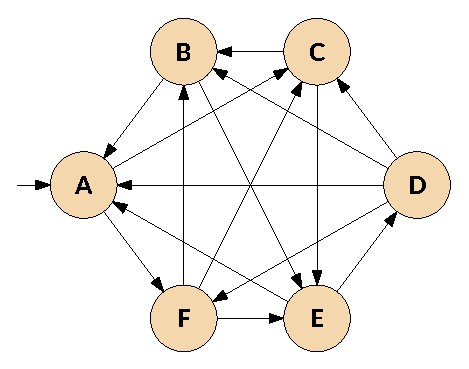
\includegraphics[]{figures/ponder_central_audition_infinitepath.eps}
\end{center}

ให้พิจารณากราฟที่กำหนดให้ เราจะเขียนโปรแกรมเพื่อเดิน (traverse) บนกราฟดังกล่าว โดยมีเงื่อนไขดังนี้
\begin{enumerate}
\item เราจะเริ่มต้นการเดินจากโหนด A
\item จากโหนดหนึ่ง ๆ เราจะเดินไปยังโหนดถัดไปเฉพาะโหนดที่มีลูกศรชี้ไปหาเสมอ

    หากมีลูกศรชี้ไปยังโหนดอื่น ๆ มากกว่า 1 โหนด ให้เลือกเดินไปโหนดถัดไป\uline{โหนดใดก็ได้}
    \uline{จากตัวเลือกนั้น ๆ} (เช่น จากโหนด B เราสามารถเดินไปยังโหนด A หรือ E โหนดใดก็ได้)
\item เราจะเดินบนกราฟนี้ไปเรื่อย ๆ ไม่มีหยุดอยู่กับที่ (เสมือนว่าโปรแกรมของเรามี infinite loop)
\end{enumerate}

\noindent
จากการเดินบนกราฟอย่างไม่สิ้นสุดตามคำอธิบายข้างต้น ข้อใดต่อไปนี้ถูกต้องบ้าง?

\begin{itemize}[label={$\square$}]
    \item \textbf{ประพจน์ P:} รับประกันว่าในการเดินดังกล่าว ``เราจะเดินพบโหนด A อนันต์ครั้ง'' 
        หรือไม่เช่นนั้น ``เราจะเดินพบโหนด D อนันต์ครั้ง''
    \item \textbf{ประพจน์ Q:} รับประกันว่าในการเดินดังกล่าว ``เราจะเดินพบโหนด B อนันต์ครั้ง'' 
        หรือไม่เช่นนั้น ``เราจะเดินพบโหนด E อนันต์ครั้ง''
    \item \textbf{ประพจน์ R:} รับประกันว่าในการเดินดังกล่าว ``เราจะเดินพบโหนด C อนันต์ครั้ง'' 
        หรือไม่เช่นนั้น ``เราจะเดินพบโหนด F อนันต์ครั้ง''
\end{itemize}

\question{}

ให้พิจารณาสมการดทางด้าน\ifpageodd{ขวา}{ซ้าย}ต่อไปนี้ โดยมีเงื่อนไขว่า
\marginnote[\baselineskip]{
    \begin{center}
        
\includegraphics[width=0.85\linewidth]{figures/ponder_central_regional_cryptarithmetic.eps}
    \end{center}
}

\begin{itemize}
\item แต่จะพจน์ (term) ของการบวกคือจำนวนเต็มที่เลขโดดแต่ละตัวถูกเขียนแทนด้วยอักขระภาษาอังกฤษ 1 ตัว
\item อักขระตัวเดียวกันแทนเลขโดดเดียวกัน อักขระที่ต่างกันแทนเลขโดดที่ไม่ซ้ำกัน
\item ไม่มีพจน์ใดที่อักขระตัวแรกแทนเลขโดด 0
\end{itemize}

\noindent
อยากทราบว่าคำว่า \textbf{\ltspc BRACKET} แทนจำนวนใด?


\newpage
\question{}

กำหนดให้มีจำนวนเต็ม ได้แก่ 1, 2, 3, \ldots, 12 

ให้แบ่งกลุ่มของจำนวนเต็มดังกล่าวออกเป็น 2 กลุ่ม\; โดยแต่ละกลุ่มจะต้องมีจำนวนเต็มอย่างน้อย 1 จำนวน\; 
จากนั้นให้หาผลคูณของจำนวนในแต่ละกลุ่ม

\medskip\noindent
\textbf{\uline{โจทย์}} อยากทราบว่า\hrsp\uline{ผลต่าง}ของ\uline{ผลคูณ}จากทั้งสองกลุ่ม 
มีค่า\uline{น้อยที่สุด}เท่าใด?

\question{}

จงศึกษาตัวอย่างโจทย์ต่อไปนี้ แล้วจึงแก้โจทย์ในช่วงท้ายของคำถาม

\smallskip\noindent
\textbf{\uline{ตัวอย่าง}}\; สมมติว่ามีลูกอมยี่ห้อหนึ่ง ถูกบรรจุขายเป็นแพ็คถุง 2 ขนาด คือแบบถุงละ 3 ลูก หรือ 5 ลูก สังเกตว่า

\begin{itemize}[before*=\small]
\item เราสามารถซื้อลูกอมให้มีลูกอม\uline{เป็นจำนวนรวม} 8 ลูกได้ 
    (คือซื้อทั้งสองแบบ แบบละ 1 ถุง แล้วนำลูกอมมาเทรวมกัน)
\item แต่เรา\uline{ไม่มี}วิธีที่สามารถซื้อลูกอมเป็นจำนวนรวม 7 ลูกพอดีได้เลย
\end{itemize}

\noindent
\textbf{\uline{โจทย์}}\; สมมติว่ามีลูกอมอีกยี่ห้อหนึ่ง ถูกบรรจุขายเป็นแพ็ค 3 ขนาด 
คือแบบถุงละ 6 ลูก หรือ 15 ลูก หรือ 40 ลูก ตามลำดับ\;
แล้วจำนวนลูกอมที่มากที่สุดที่เรา\uline{ไม่สามารถ}หาวิธีซื้อให้พอดีจากการผสมแพ็คลูกอมทั้ง 3 แบบนี้ มีจำนวนลูกอมเท่าใด?

\question{}

ในปัจจุบัน เงินตราที่นิยมใช้กันแพร่หลายในประเทศไทยประกอบไปด้วยเหรียญกษาปณ์หรือธนบัตรชนิดราคา\; 
1 บาท, 2 บาท, 5 บาท, 10 บาท, 20 บาท, 50 บาท, 100 บาท, 500 บาท และ 1000 บาท ตามลำดับ

สมมติว่าเราต้องการชำระยอดหนี้ก้อนหนึ่งซึ่งมีมูลค่า $d$ บาท
โดยมี\emph{{\hrsp}เป้าหมาย{\hrsp}}ว่าจะต้องใช้เงินตราเป็นจำนวน\uline{น้อยที่สุด}เพื่อชำระหนี้ดังกล่าว\uline{ให้พอดี}\;
สังเกตว่าเราสามารถใช้ \textbf{Greedy algorithm} ดังต่อไปนี้ เพื่อบรรลุ{\hrsp}\emph{เป้าหมาย}{\hrsp}ดังกล่าวได้\hrsp%
\sidenote{%
    หมายความว่า \textbf{Greedy algorithm} ให้ผลลัพธ์เป็น \emph{optimal} สำหรับเงินตราที่ระบุไว้ข้างต้น
} 
ไม่ว่ายอดหนี้ $d$ จะมีมูลค่ากี่บาทก็ตาม

\begin{quote}
    \textbf{Greedy algorithm.} เราจะเลือกเหรียญกษาปณ์หรือธนบัตรที่มีมูลค่ามากที่สุดที่เป็นไปได้ที่ไม่เกินยอดหนี้ นำไปหักจากยอดหนี้ 
    ทำเช่นนี้ไปเรื่อย ๆ จนกว่ายอดหนี้จะลดลงเหลือ 0 บาท

    ยกตัวอย่างเช่น หากเราต้องการชำระหนี้มูลค่า $d = \mathrm{94}$ บาท เราสามารถจ่ายด้วยเหรียญกษาปณ์หรือธนบัตรที่มีมูลค่า 
    $\mathrm{50+20+20+2+2}$ ตามลำดับ ซึ่งหมายความว่าเราใช้จำนวนเงินตรา 5 อัน ซึ่งน้อยที่สุดที่เพียงพอจะชำระหนี้ดังกล่าวพอดี
\end{quote}

\uline{อย่างไรก็ดี} สมมติว่าวันหนึ่ง\,ประเทศไทยจะเพิ่มเหรียญกษาปณ์หรือธนบัตรชนิดราคาใหม่จำนวน
1 ชนิดราคาเข้ามาในระบบ สังเกตว่า

\begin{itemize}[before*=\small]

\item ถ้าสมมติว่าประเทศไทยตัดสินใจเพิ่มเหรียญกษาปณ์ชนิดราคา 4 บาทเข้ามาในระบบ แล้ว \textbf{Greedy algorithm} 
ข้างต้นจะไม่รับประกันว่าจะให้ผลลัพธ์ที่ optimal เสมอไป\; 
(เช่น หากต้องการชำระเงิน $d = \mathrm{8}$ บาท \textbf{Greedy algorithm} จะจ่ายด้วยเหรียญ $\mathrm{5+2+1}$ บาทตามลำดับ 
แทนการใช้วิธี $\mathrm{4+4}$ บาทที่ใช้จำนวนเงินตราน้อยกว่า)

\item แต่ถ้าเราเพิ่มเหรียญกษาปณ์ชนิดราคา 3 บาทแล้ว \textbf{Greedy algorithm} จะยังคงให้จำนวนเงินตราที่ optimal 
อยู่ไม่ว่ายอดหนี้ $d$ จะมีมูลค่าเท่าใดก็ตาม

\end{itemize}

\uline{จงหาเงินตราที่มีชนิดราคาสูงที่สุด 1 ชนิดราคา} ที่เมื่อเพิ่มเข้ามาในระบบแล้วจะทำให้ 
\textbf{Greedy algorithm} ให้ผลลัพธ์ไม่เป็น optimal สำหรับยอดหนี้บางจำนวน\sidenote[][-\baselineskip]{%
    พร้อมทั้งยกตัวอย่างค้านว่า ยอดหนี้ $d$ มูลค่าเท่าใดที่ทำให้  \textbf{Greedy algorithm} ให้ผลลัพธ์ที่ไม่เป็น optimal
}


\newpage
\question{}

พิซซ่าถาดหนึ่งถูกตัดแบ่งด้วยรัศมีออกเป็นพิซซ่าชิ้นย่อย ๆ 8 ชิ้นที่มาขนาดเท่า ๆ กัน\;
ต่อจากนั้นพิซซ่า\uline{แต่ละชิ้น}ย่อยทุกชิ้นจะถูกทาด้วยซอส 1 ใน 3 ชนิด (ได้แก่ ซอสขาว ซอสแดง หรือซอสน้ำตาล)

\medskip\noindent
\textbf{\uline{นิยาม}} พิซซ่าสองถาดจะมีหน้าตา\uline{แบบเดียวกัน} 
ก็ต่อเมื่อ หากสามารถหมุนถาดพิซซ่าถาดหนึ่งให้มีหน้าตาเหมือนกันพิซซ่าอีกถาดหนึ่งได้

\begin{fullwidth}
    \begin{multicols}{2}
        \begin{center}
            
\includegraphics[width=0.85\linewidth]{figures/ponder_central_regional_pizzapaint_01.eps}\\
            ตัวอย่างของพิซซ่าที่หน้าตา\uline{เหมือนกัน}        
            
            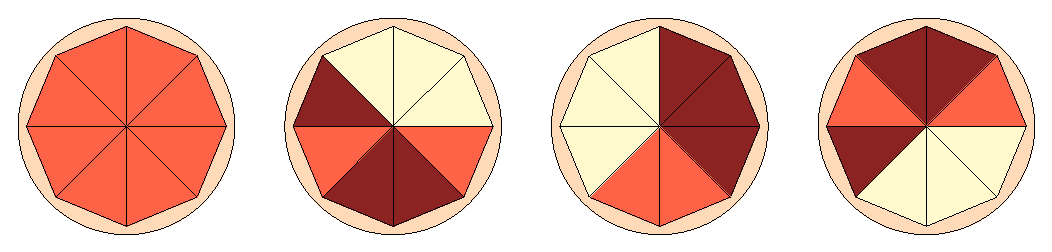
\includegraphics[width=0.85\linewidth]{figures/ponder_central_regional_pizzapaint_02.eps}\\
            ตัวอย่างของพิซซ่าที่หน้าตา\uline{แตกต่างกันทั้งหมด}
        \end{center}
        
    \end{multicols}
\end{fullwidth}

\medskip\noindent
\textbf{\uline{โจทย์}} อยากทราบว่าเราจะได้ถาดพิซซ่าที่หน้าตามีการทาซอสออกมาแตกต่างกันทั้งหมดกี่แบบ?


\question{}

จงเติมจำนวนเต็ม 1 ถึง 16 ลงในตารางขนาด $\mathrm{4} \times \mathrm{4}$ 
มาอย่างน้อย 1 วิธีซึ่งสอดคล้องกับเงื่อนไขดังต่อไปนี้
\marginnote[\baselineskip]{
    \centering
    
\includegraphics[width=0.7\linewidth]{figures/ponder_national_fourbyfour.eps}
}

\begin{itemize}
\item จำนวนใน\uline{แต่ละช่อง}ต้อง\uline{ไม่ซ้ำกัน}
\item จำนวนใน\uline{แต่ละแถว} จะต้องเรียงลำดับจากน้อยไปมาก จาก\uline{ซ้ายไปขวา}
\item จำนวนใน\uline{แต่ละคอลัมน์} จะต้องเรียงลำดับจากน้อยไปมาก จาก\uline{บนลงล่าง}
\item สำหรับทุก $k \in \{\mathrm{1, 2, 3, 4}\}$\; ผลรวมของจำนวนในแถวที่ $k$ (นับจากบน) จะต้อง\uline{เท่ากับ}
    ผลรวมของจำนวนในคอลัมน์ที่ $k$ (นับจากซ้าย)
\end{itemize}

\question{}

กำหนดให้ \lstinline{validate_array(A)} คือฟังก์ชันที่รับ input argument
เป็น 0-indexed array \lstinline{A} ของจำนวนเต็ม\;
และให้ output result เป็นค่า boolean ที่เป็น \lstinline{true} หรือ \lstinline{false} เท่านั้น\;
ฟังก์ชันดังกล่าว สามารถเขียนเป็น pseudocode ได้ดังนี้
\begin{fullwidth}
\vspace*{-\baselineskip}    
\begin{lstlisting}
function validate_array(A[0...n-1]):
    return (0 ≤ A[i] ≤ n-1 and A[i] == A[A[i]] for each i := 0 to n-1)  <%\SuppressNumber%>
           and (A[i-1] ≤ A[i] for each i := 1 to n-1)  <%\ReactivateNumber%>
end
\end{lstlisting}
\end{fullwidth}

\smallskip\noindent
ตัวอย่างของการเรียกใช้ฟังก์ชันข้างต้น
\begin{itemize}[itemsep=0pt]
\item \lstinline|validate_array(A = [0, 1, 1, 3])  # => true|
\item \lstinline|validate_array(A = [2, 2, 2, 2])  # => true|
\item \lstinline|validate_array(A = [1, 2, 3, 3])  # => false|
\item \lstinline|validate_array(A = [3, 1, 1, 3])  # => false|
\end{itemize}

\textbf{\uline{โจทย์}}\; จงหา\uline{จำนวนรูปแบบ}ทั้งหมดของ input array \lstinline|A| 
ที่มีจำนวนสมาชิก 20 ตัวที่ทำให้ \lstinline|validate_array(A)| คืนค่าออกมาเป็น \lstinline|true|?


\newpage
\question{}

เราต้องการแขวนกรอบรูปอันหนึ่งด้วยเชือก 1 เส้นที่ร้อยจากขอบซ้ายของรูป คล้องเหนือหมุดบนกำแพงบางอัน 
แล้วมาร้อยเชื่อมกับขอบขวาของรูป

\marginnote[\baselineskip]{%
    \centering

    \noindent
    
\includegraphics[scale=0.5]{figures/ponder_national_picturehang_01.eps}
    \hfill
    
\includegraphics[scale=0.5]{figures/ponder_national_picturehang_02.eps}
    
    \bigskip\noindent
    
\includegraphics[scale=0.5]{figures/ponder_national_picturehang_03.eps}
    \hfill
    
\includegraphics[scale=0.5]{figures/ponder_national_picturehang_04.eps}
}

\medskip\noindent
\textbf{\uline{ตัวอย่าง}\; หมุด 2 ตัว} ---
สมมติว่าเราเลือกที่จะแขวนรูปโดยการร้อยเชือกกับหมุด 2 ตัวในรูปแบบต่าง ๆ ดังนี้
\begin{itemize}[before*=\small]
\item \textbf{รูปสีฟ้า:} หากเราแขวนรูปด้วยวิธีปกติ (ดังรูปสีฟ้า) เราพบว่าหากหมุด\uline{ตัวใดตัวหนึ่ง}ถูกดึงออกไป 
    หมุดอีกตัวหนึ่งจะยังสามารถรั้งกรอบภาพ\uline{ไม่ให้ตก}ตามแรงโน้มถ่วงได้
\item \textbf{รูปสีเขียว:} แต่หากเราแขวนอีกแบบหนึ่ง (ดังรูปสีเขียว) เราพบว่ากรอบภาพจะยังคงแขวนได้เช่นกัน
    แต่หากหมุดตัวใดตัวหนึ่งถูกดึงออกไป กรอบภาพจะ\uline{หลุดลงมาทันที}แม้ว่าหมุดอีกตัวจะยังยึดกำแพงอยู่ก็ตาม
\end{itemize}

\noindent
\textbf{\uline{โจทย์}\; หมุด 3 ตัว} ---
หากเรามีหมุดสามอัน คือ A, B, C เรียงจากซ้ายไปขวา (ดู\textbf{รูปสีส้ม}ประกอบ) 
เราต้องการร้อยเชือกรอบหมุดให้สอดคล้องกับเงื่อนไขต่อไปนี้
\begin{itemize}
\item หากดึงหมุด A หรือหมุด C อันใดอันหนึ่ง รูปจะยังรั้งไว้ได้ ไม่หล่นลงมา
\item หากดึงหมุด B หมุดเดียว รูปจะหล่นลงมาทันที
\item หากดึงทั้งหมุด A และหมุด C ทั้งสองหมุด รูปจะหล่นลงมาเช่นกัน
\end{itemize}

\noindent
จงหาวิธีแขวน{\hrsp}\textbf{รูปสีส้ม}{\hrsp}ที่สอดคล้องกับเงื่อนไขข้างต้น\hrsp%
\sidenote{%
    นอกจากนี้ ยังมี\uline{ข้อห้าม}เกี่ยวกับการแขวนรูปดังนี้
    \begin{itemize}
        \item \uline{ห้าม}ใช้เชือกคล้องกันเอง (ดังเช่น{\hrsp}\textbf{รูปสีแดง}\hrsp) ในรูปนี้ให้ถือว่าเชือกขดทับกันแต่ไม่ไขว้กัน 
            ซึ่งแปลว่ารูปจะไม่ถูกแขวนได้สำเร็จแต่แรก 
        \item นอกจากนั้น \uline{ห้าม}มัดเชือกกันเองเป็นปมเพื่อแขวนรูป
    \end{itemize}
}

% https://firebasestorage.googleapis.com/v0/b/kbtg-techjam-code-questions.appspot.com/o/questions%2F42e9879c-9f26-4db2-874b-a047489f5286%2FHangingFrame.png?alt=media&token=d48a294b-0c99-4b49-9099-35d7e3936dff
\question{}

มีตู้เซฟอยู่ตู้หนึ่ง ตู้เซฟนี้ถูกล็อกด้วยหมายเลขปริศนา \lstinline{Q} ซึ่งมีความยาว 6 หลัก 
(เราเรียก \lstinline{Q} ว่า\emph{\hrsp รหัสผ่านจริง\hrsp})

ทุก ๆ ครั้งที่เราป้อนรหัสเซฟเพื่อเปิดตู้เซฟตู้นี้ หากเราป้อนรหัสไม่ถูกต้อง ตู้เซฟจะมีเสียงร้องพร้อมทั้งยังมีข้อความตอบกลับ
(response message) ว่า
\begin{quote}
    \centering
    เลขโดดที่อยู่ติดกันที่ยาวที่สุดที่ปรากฏทั้งในรหัสผ่านจริง \lstinline{Q} \\
    และ\emph{\hrsp รหัสผ่านที่ป้อนผิด\hrsp}นั้นมีความยาวเท่าใด\hrsp%
    \sidenote{%
        พูดอีกนัยหนึ่งคือ response message จะเป็นความยาวของ 
        \textbf{Longest common substring} (\lstinline{LCS})
        ระหว่างรหัสผ่านจริง \lstinline{Q} กับ\emph{\hrsp รหัสผ่านที่ป้อนผิด\hrsp}
        
        \smallskip
        \textbf{ตัวอย่าง}\; สมมติว่ารหัสผ่านจริงของตู้เซฟคือ 
        \begin{center}
            \lstinline{Q = 123456} 
        \end{center}
        แต่เราป้อนรหัสตู้เซฟเป็น
        \begin{center}
            \lstinline{A = 134579}
        \end{center}
        แล้วตู้เซฟจะมี response message ตอบกลับออกมาเป็น
        \begin{center}
            \lstinline{LCS(A, Q) = 3}
        \end{center}
    }
\end{quote} 

ต่อไปนี้คือประวัติของการลองป้อนรหัสเซฟแก่ตู้เซฟนี้ทั้งสิ้น 9 ครั้ง พร้อมทั้ง response message ในแต่ละครั้ง
\begin{center}
    \smallskip
    \begin{tabular}{@{\quad}c@{\qquad\qquad}c@{\quad}}
        \toprule
        รหัสผ่านที่ป้อน \lstinline|A| & ข้อความตอบกลับ \lstinline|LCS(A, Q)|  \\
        \midrule
        \verb|027292| & \verb|1| \\
        \verb|135135| & \verb|0| \\
        \verb|257015| & \verb|2| \\
        \verb|362447| & \verb|1| \\
        \verb|470619| & \verb|3| \\
        \verb|560968| & \verb|1| \\
        \verb|674669| & \verb|1| \\
        \verb|822642| & \verb|1| \\
        \verb|903287| & \verb|3| \\
        \bottomrule
    \end{tabular}
    \smallskip
\end{center}

จงหารหัสผ่านจริง \lstinline{Q} ของตู้เซฟนี้จากข้อมูลข้างต้น


\newpage
\question{}

ปัญหา \textbf{Traveling salesperson problem} (TSP) คือปัญหากราฟที่มีเป้าหมายเพื่อค้นหาเส้นทางจากโหนดหนึ่ง ๆ 
ไปเยือนโหนดอื่น ๆ ทุกโหนด ก่อนกลับมายังโหนดเริ่มต้น โดยใช้ระยะทางรวมน้อยที่สุด

สำหรับโจทย์ข้อนี้ให้พิจาณา Greedy algorithm เพื่อแก้ปัญหา TSP ข้างต้น ซึ่งมีขั้นตอนวิธีดังนี้\hrsp%
\sidenote[][-\baselineskip]{%
    อัลกอริทึมนี้มีความเป็น non-deterministic
    เนื่องจากอัลกอริทึมมีการตัดสินใจแบบ arbitrary ได้เมื่อมีตัวเลือกปรากฏขึ้น ซึ่งมีผลทำให้ได้คำตอบที่แตกต่างออกไป

    ขั้นตอนของอัลกอริทึมดังกล่าวที่มีความเป็น non-deterministic จะมีเครื่องหมายดอกจันกำกับ
}
\begin{enumerate}
\item เริ่มต้นจาก\uline{โหนดใดก็ได้}*
\item \label{item:ponder_national_greedytsp_anynearest} 
    จากโหนดปัจจุบัน ให้เลือกไปเยือนโหนดถัดไปที่อยู่ใกล้ที่สุดที่ยังไม่เคยเดินทางไปเยือน \\
    \textbf{หมายเหตุ:} หากมีหลายโหนดที่สอดคล้องกับเงื่อนไขข้างต้น ให้เลือกไปเยือน\uline{โหนดใดก็ได้}
    ในบรรดาโหนดเหล่านั้น*
\item เมื่อกระทำตามข้อ \ref*{item:ponder_national_greedytsp_anynearest} จนเยือนครบทุกโหนดแล้ว 
    ให้เดินกลับไปยังโหนดที่เป็นจุดเริ่มต้น
\end{enumerate}

อย่างไรก็ดี Greedy algorithm นี้\uline{ไม่รับประกัน}ว่าจะให้คำตอบที่ดีที่สุด (หรือ optimal solution) เสมอไป\;
โจทย์ข้อนี้เราจะพิจารณา\uline{หาตัวอย่างค้าน}ที่ Greedy algorithm ข้างต้นให้ผลลัพธ์ที่แย่มากเป็นพิเศษ 

\marginnote{%
    \begin{center}
        
\includegraphics[scale=0.75]{figures/ponder_national_greedytsp_02.eps} \\ 
        ({\hrsp}a{\hrsp})
        
        \vspace{2\baselineskip}
        
\includegraphics[scale=0.75]{figures/ponder_national_greedytsp_03.eps} \\ 
        ({\hrsp}b{\hrsp})
        
        \vspace{2\baselineskip}
        
\includegraphics[scale=0.75]{figures/ponder_national_greedytsp_04.eps} \\ 
        ({\hrsp}c{\hrsp})
    \end{center}
}
\begin{center}
    \medskip
    
\includegraphics[]{figures/ponder_national_greedytsp_01.eps}
\end{center}

\noindent
\textbf{\uline{เคสตัวอย่าง}} ให้พิจารณากราฟข้างต้น ซึ่งประกอบด้วยจุดบน Euclidean space 
ที่เรียงเป็นตารางสี่เหลี่ยมผืนผ้า 3 แถว แถวละ 4 จุด\; นอกจากนั้นแต่ละแถวและแต่ละคอลัมน์ห่างกัน 1 หน่วย

\begin{itemize}
\item หากเราโชคดีหน่อย Greedy algorithm อาจจะค้นพบเส้นทาง ({\hrsp}a{\hrsp}) 
    ที่แสดงทางด้าน\ifpageodd{ขวา}{ซ้าย}มือ 
    เส้นทางดังกล่าวมีระยะทางเท่ากับ $\mathrm{12}$ หน่วย ซึ่งเป็น optimal solution
\item แต่หากโชคไม่ค่อยดี Greedy algorithm มีโอกาสพบเส้นทางอื่นเช่น ({\hrsp}b{\hrsp}) หรือ ({\hrsp}c{\hrsp}) 
    ซึ่งมีระยะทางรวมเท่ากับ $\mathrm{14}$ หน่วย 
    และ $\mathrm{11} + \sqrt{\mathrm{5}}\approx\mathrm{13.236}$ หน่วยตามลำดับ
\end{itemize}

\noindent
จงหาเส้นทางที่ Greedy algorithm นี้มีโอกาสค้นพบ ที่มีระยะทางมากกว่า $\dfrac{\mathrm{160}}{\mathrm{9}}$ หน่วย


\question{}

จงพิจารณาระบบการถ่ายเทพลังงานในระบบห่วงโซ่อาหารของสัตว์กลุ่มหนึ่ง 
โดยที่สัตว์ทุกตัวในกลุ่มนี้มีโอกาสเป็นทั้งผู้ล่าและเหยื่อกับสัตว์ตัวอื่น ๆ ได้ทุกตัว
\begin{itemize}
\item กำหนดให้สัตว์ทุกตัวมี\uline{พลังงานสะสมเริ่มต้น}ในร่างกาย 1,000,000 KCal
\item เมื่อเกิดการล่าเหยื่อขึ้น หากสัตว์ A จับสัตว์ B เป็นอาหารแล้วพบว่า B จะเสียชีวิตไป 
    และ A จะได้รับถ่ายทอดพลังงานสะสม\uline{ครึ่งหนึ่ง}จาก B\hrsp%
    \sidenote{%
        \textbf{หมายเหตุ}\; เราสมมติว่าสัตว์แต่ละตัวจะไม่เสียพลังงานใด ๆ กับกิจกรรมอื่น ๆ เลย
        พลังงานจะหายไปจากระบบจากการที่เหยื่อถูกบริโภคเท่านั้น
    }
\item สัตว์ทุกตัวในระบบจะจับเหยื่อตัวอื่น ๆ เป็นอาหารได้ไม่เกิน 3 ตัว
\end{itemize}

หากในตอนแรกมีสัตว์ในระบบนิเวศนี้ทั้งสิ้น 1,000 ตัว แล้วจึงเกิดการล่ากันเองขึ้นจนเหลือสัตว์ที่อยู่รอดตัวเดียว 
สัตว์ตัวดังกล่าวนี้จะมีพลังงานสะสมตอนท้าย\uline{อย่างน้อยที่สุด}และ
\uline{อย่างมากที่สุด}กี่ KCal? ({\hrsp}ให้ตอบเป็นจำนวนเต็มโดย\uline{ปัดเศษทิ้ง}{\hrsp})


\newpage
\question{}

จงศึกษาตัวอย่างโจทย์ต่อไปนี้ แล้วจึงแก้โจทย์ในช่วงท้ายของคำถาม

\marginnote{%
    \centering
    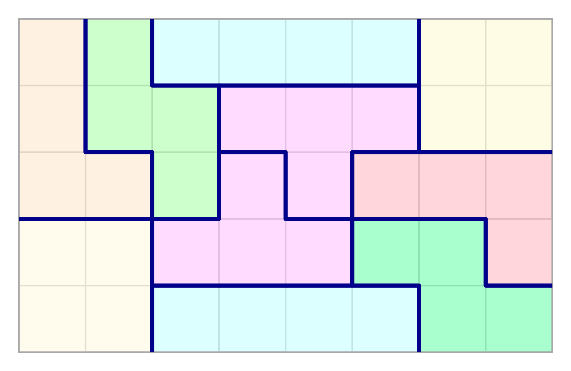
\includegraphics[width=0.98\linewidth]{figures/ponder_national_tetris.eps}
    \vspace{\baselineskip}
}

\smallskip\noindent
\textbf{\uline{ตัวอย่าง}} พิจารณารูปที่ปรากฏทาง\ifpageodd{ขวา}{ซ้าย}มือ 
เป็นพื้นที่สี่เหลี่ยมผืนผ้าขนาด $\mathrm{8 \times 5}$ หน่วย 
ซึ่งถูกตัดแบ่งออกเป็นชิ้นส่วน TETRIS{\textregistered} ประกอบกัน 10 ชิ้น ด้วยการขีดเส้นปากกาดังรูป
(แสดงด้วยเส้นสีน้ำเงินทึบภายในกรอบสี่เหลี่ยม)\; พบว่าความยาวเส้นปากกาดังกล่าวคือ 35 หน่วย\hrsp%
\sidenote{%
    \textbf{หมายเหตุ}\; ความยาวของเส้นปากกา เรานับเฉพาะเส้นที่คั่นระหว่างชิ้นส่วน 
    TETRIS{\textregistered} สองชิ้น และไม่นับเส้นกรอบ
}

สังเกตว่า หากพื้นที่สี่เหลี่ยมผืนผ้านี้ถูกแบ่งเป็นชิ้นส่วน TETRIS{\textregistered} ในรูปแบบที่ต่างออกไป 
อาจจะต้องขีดเส้นปากกาที่มีความยาวรวมมากกว่าหรือน้อยกว่า 35 หน่วยก็ได้

\smallskip\noindent
\textbf{\uline{โจทย์}}\; ให้พิจารณาพื้นที่สี่เหลี่ยมผืนผ้าขนาด $\mathrm{12 \times 9}$ หน่วย 
หากเราใช้ปากกขีดเส้น\uline{ภายใน}
กรอบสี่เหลี่ยม เพื่อแบ่งให้พื้นที่ว่างในกรอบเป็นชิ้นส่วน TETRIS{\textregistered} จำนวน 27 ชิ้น

จงคำนวณหาว่า เส้นปากกาที่ขีดในกรอบสี่เหลี่ยมดังกล่าวจะมีความยาวรวม\uline{น้อยที่สุด}และ
\uline{มากที่สุด}กี่หน่วย?


\question{}

ในโรงเรียนประถมศึกษาแห่งหนึ่ง มีห้องเรียนชั้น ป.1 อยู่ 2 ห้อง ได้แก่ห้องทานตะวัน และห้องกุหลาบ

เด็กชาย K เรียนอยู่ในห้องทานตะวัน และมีเพื่อนสนิทอยู่ 8 คน ได้แก่ A, B, C, D, E, F, G และ H\;\;
บางคนเรียนอยู่ห้องทานตะวันเช่นเดียวกับเด็กชาย K \;
ส่วนบางคนเรียนอยู่ห้องกุหลาบ คนละห้องกับเด็กชาย K

ต่อไปนี้คำบอกกล่าวของครูใหญ่ทั้งสิ้น 14 ประโยค

\begin{multicols}{2}
    \begin{enumerate}
        \item A กับ B เรียนอยู่คนละห้องกัน
        \item B กับ C เรียนอยู่คนละห้องกัน
        \item C กับ D เรียนอยู่คนละห้องกัน
        \item D กับ E เรียนอยู่คนละห้องกัน
        \item E กับ A เรียนอยู่คนละห้องกัน
        \item A กับ F เรียนอยู่คนละห้องกัน
        \item F กับ G เรียนอยู่คนละห้องกัน
        \item G กับ H เรียนอยู่คนละห้องกัน
        \item H กับ D เรียนอยู่คนละห้องกัน
        \item D กับ B เรียนอยู่คนละห้องกัน
        \item B กับ E เรียนอยู่คนละห้องกัน
        \item E กับ C เรียนอยู่คนละห้องกัน
        \item C กับ K เรียนอยู่คนละห้องกัน
        \item K กับ G เรียนอยู่คนละห้องกัน
    \end{enumerate}
\end{multicols}

ในบรรดา 14 ประโยคข้างต้น มี \uline{2 ประโยคที่ไม่เป็นความจริง} 
จงพิจารณาข้อมูลข้างต้นแล้วตอบคำถามต่อไปนี้
\begin{itemize}
\item ประโยคใดเป็นเท็จบ้าง?
\item ใครเรียนอยู่ห้องทานตะวันเช่นเดียวกับเด็กชาย K บ้าง?
\end{itemize}

